\documentclass[
  % -- opções da classe memoir --
  12pt,				% tamanho da fonte
  %openright,			% capítulos começam em pág ímpar (insere página vazia caso preciso)
  %twoside,			% para impressão em verso e anverso. Oposto a oneside
  oneside,			% para impressão em verso e anverso. Oposto a oneside
  a4paper,			% tamanho do papel. 
  % -- opções da classe abntex2 --
  %chapter=TITLE,		% títulos de capítulos convertidos em letras maiúsculas
  %section=TITLE,		% títulos de seções convertidos em letras maiúsculas
  %subsection=TITLE,	% títulos de subseções convertidos em letras maiúsculas
  %subsubsection=TITLE,% títulos de subsubseções convertidos em letras maiúsculas
  % -- opções do pacote babel --
  english,			% idioma adicional para hifenização
  brazil,				% o último idioma é o principal do documento
  % -- opções da classe ime-abntex2 --
  %brasao,
]{ime-abntex2}


% ---
% PACOTES
% ---

\usepackage[utf8]{inputenc}		% Codificacao do documento (conversão automática dos acentos)
\usepackage{cmap}			% Mapear caracteres especiais no PDF
\usepackage{lmodern}			% Usa a fonte Latin Modern
\usepackage{amsmath}			% Para usar blocos como "gather" de escrever matemática
%\usepackage{amsfonts}			% Para usar fontes ams
%\usepackage{times}			% Usa a fonte Times
\usepackage[T1]{fontenc}		% Selecao de codigos de fonte.
%\usepackage{lastpage}			% Usado pela Ficha catalográfica
\usepackage{indentfirst}		% Indenta o primeiro parágrafo de cada seção.
\usepackage{color}			% Controle das cores
\usepackage{graphicx}			% Inclusão de gráficos
\usepackage{algorithm2e}		% Para escrever algorítimos
\usepackage{lscape}			% Para usar landscape
\usepackage{amsthm}			% Para usar Definições e lemas
\usepackage{amssymb}			% \mathbb{•}
\usepackage{caption}			% dependencia de subcaption
%\usepackage{subcaption}			% Para usar \begin{subfigure} e colocar figuras (a) e (b) lado a lado
\usepackage{listings}			% Para usar \lstinputlisting e incluir código
\newtheorem{teo}{Teorema}[section]	%Renomear o comando
\newtheorem{defi}[teo]{Definição}
% o seguinte é necessário para corrigir um bug no algorithm2e
% http://tex.stackexchange.com/questions/113325/problem-with-algorithm2e-and-portuguese-option
\SetKwFor{Para}{para}{fa\c{c}a}{fim para}
% não era pra precisar do seguinte, mas precisa para traduzir a captions dos algoritmos
\renewcommand{\algorithmcfname}{Algoritmo}%
% ---

% ---
% Pacotes de citacoes
% ---
% O seguinte serve para mostrar as referencias reversas na bibliografia
% \usepackage[brazilian,hyperpageref]{backref}	 % Paginas com as citações na bibl
\usepackage[alf]{abntex2cite}	% Citações padrão ABNT

% --- 
% CONFIGURAÇÕES DE PACOTES
% --- 

% ---
% Configurações do pacote backref
% Usado sem a opção hyperpageref de backref
%\renewcommand{\backrefpagesname}{Citado na(s) página(s):~}
% Texto padrão antes do número das páginas
%\renewcommand{\backref}{}
% Define os textos da citação
%\renewcommand*{\backrefalt}[4]{
%	\ifcase #1 %
%		Nenhuma citação no texto.%
%	\or
%		Citado na página #2.%
%	\else
%		Citado #1 vezes nas páginas #2.%
%	\fi}%
% ---

% as imagens ficam nesse diretório
\graphicspath{{img/}}


% ---
% Informações de dados para CAPA e FOLHA DE ROSTO
% ---
\titulo{Técnicas de IA Aplicadas a Sistemas Multiagentes Cooperativos e
Competitivos}
\autor{Jan Segre\\Victor Bramigk}
\local{Rio de Janeiro}
\data{Julho de 2014}
\orientador{Paulo Fernando Ferreira Rosa}{Ph.D., do IME}
\coorientador{Bruno Eduardo Madeira}%{M.Sc., do IME}
\instituicao{%
  Instituto Militar de Engenharia
  \par
  Seção de Computação
  \par
  Graduação em Engenharia de Computação
}
\tipotrabalho{Iniciação à Pesquisa}
% O preambulo deve conter o tipo do trabalho, o objetivo,
% o nome da instituição e a área de concentração 
\preambulo{Projeto Final de Curso de Graduação em Engenharia de Computação do
Instituto Militar de Engenharia.}
% ---


% ---
% Configurações de aparência do PDF final

% alterando o aspecto da cor azul
%\definecolor{blue}{RGB}{41,5,195}
\definecolor{blue}{RGB}{0,0,0}

% informações do PDF
\makeatletter
\hypersetup{%
  %pagebackref=true,
  pdftitle={\@title},
  pdfauthor={\@author},
  pdfsubject={\imprimirpreambulo},
  pdfcreator={LaTeX with abnTeX2},
  pdfkeywords={ime}{robocup}{analise}{logs}{rede neural},
  colorlinks=true,		% false: boxed links; true: colored links
  linkcolor=blue,			% color of internal links
  citecolor=blue,			% color of links to bibliography
  filecolor=magenta,		% color of file links
  urlcolor=blue,
  bookmarksdepth=4
}
\makeatother
% ---

% ---
% Espaçamentos entre linhas e parágrafos 
% ---

% O tamanho do parágrafo é dado por:
%\setlength{\parindent}{1.3cm}

% Controle do espaçamento entre um parágrafo e outro:
%\setlength{\parskip}{0.2cm}  % tente também \onelineskip
\setlength{\parskip}{\onelineskip}

% ---
% compila o indice
% ---
\makeindex
% ---

% ----
% Início do documento
% ----
\begin{document}

% Retira espaço extra obsoleto entre as frases.
%\frenchspacing

% ----------------------------------------------------------
% ELEMENTOS PRÉ-TEXTUAIS
% ----------------------------------------------------------
% \pretextual

% ---
% Capa
% ---
\imprimircapa
%\input{pre_textuais/capa}
% ---

% ---
% Folha de rosto
% (o * indica que haverá a ficha bibliográfica)
% ---
\imprimirfolhaderosto*
%\input{pre_textuais/folha_de_rosto}
% ---

% ---
% Inserir a ficha bibliografica
% ---

% Isto é um exemplo de Ficha Catalográfica, ou ``Dados internacionais de
% catalogação-na-publicação''. Você pode utilizar este modelo como referência. 
% Porém, provavelmente a biblioteca da sua universidade lhe fornecerá um PDF
% com a ficha catalográfica definitiva após a defesa do trabalho. Quando estiver
% com o documento, salve-o como PDF no diretório do seu projeto e substitua todo
% o conteúdo de implementação deste arquivo pelo comando abaixo:
%
% \begin{fichacatalografica}
%     \includepdf{fig_ficha_catalografica.pdf}
% \end{fichacatalografica}
\imprimirfichacatalografica
{629.892}
{S455h}
{Segre, Jan}
{Projeto de Fim de Curso (PFC)}
{%
  1. Curso de engenharia da computação - Projeto Final de Curso.
  2. Robótica.
  3. Minimax.
  I. Bramigk, Victor.
  II. Rosa, Paulo Fernando Ferreira.
  III. Bruno Eduardo Madeira.
  IV. \@title.
  V. Instituto Militar de Engenharia.
}
{Técnicas de IA aplicadas a sistemas multiagentes cooperativos e
competitivos}
% ---

% ---
% Inserir errata
% ---
%\begin{errata}
%Elemento opcional da \citeonline[4.2.1.2]{NBR14724:2011}. Exemplo:
%
%\vspace{\onelineskip}
%
%FERRIGNO, C. R. A. \textbf{Tratamento de neoplasias ósseas apendiculares com
%reimplantação de enxerto ósseo autólogo autoclavado associado ao plasma
%rico em plaquetas}: estudo crítico na cirurgia de preservação de membro em
%cães. 2011. 128 f. Tese (Livre-Docência) - Faculdade de Medicina Veterinária e
%Zootecnia, Universidade de São Paulo, São Paulo, 2011.
%
%\begin{table}[htb]
%\center
%\footnotesize
%\begin{tabular}{|p{1.4cm}|p{1cm}|p{3cm}|p{3cm}|}
%  \hline
%   \textbf{Folha} & \textbf{Linha}  & \textbf{Onde se lê}  & \textbf{Leia-se}  \\
%    \hline
%    1 & 10 & auto-conclavo & autoconclavo\\
%   \hline
%\end{tabular}
%\end{table}
%
%\end{errata}
% ---

% ---
% Inserir folha de aprovação
% ---
%
% Isto é um exemplo de Folha de aprovação, elemento obrigatório da NBR
% 14724/2011 (seção 4.2.1.3). Você pode utilizar este modelo até a aprovação
% do trabalho. Após isso, substitua todo o conteúdo deste arquivo por uma
% imagem da página assinada pela banca com o comando abaixo:
%
% \includepdf{folhadeaprovacao_final.pdf}
%
\convidadoum{Bruno Eduardo Madeira}{M.Sc., do IME}
\convidadodois{Julio Cesar Duarte}{D.Sc., do IME}
\imprimirfolhadeaprovacao{5 de setembro de 2014}
% ---

% ---
% Dedicatória
% ---
%\begin{dedicatoria}
%   \vspace*{\fill}
%   \centering
%   \noindent
%   \textit{ Este trabalho é dedicado às crianças adultas que,\\
%   quando pequenas, sonharam em se tornar cientistas.} \vspace*{\fill}
%\end{dedicatoria}
% ---

% ---
% Agradecimentos
% ---
%\begin{agradecimentos}
%Os agradecimentos principais são direcionados à Gerald Weber, Miguel Frasson,
%Leslie H. Watter, Bruno Parente Lima, Flávio de Vasconcellos Corrêa, Otavio Real
%Salvador, Renato Machnievscz\footnote{Os nomes dos integrantes do primeiro
%projeto abn\TeX\ foram extraídos de
%\url{http://codigolivre.org.br/projects/abntex/}} e todos aqueles que
%contribuíram para que a produção de trabalhos acadêmicos conforme
%as normas ABNT com \LaTeX\ fosse possível.
%
%Agradecimentos especiais são direcionados ao Centro de Pesquisa em Arquitetura
%da Informação\footnote{\url{http://www.cpai.unb.br/}} da Universidade de
%Brasília (CPAI), ao grupo de usuários
%\emph{latex-br}\footnote{\url{http://groups.google.com/group/latex-br}} e aos
%novos voluntários do grupo
%\emph{\abnTeX}\footnote{\url{http://groups.google.com/group/abntex2} e
%\url{http://abntex2.googlecode.com/}}~que contribuíram e que ainda
%contribuirão para a evolução do \abnTeX.
%
%\end{agradecimentos}
% ---

% ---
% Epígrafe
% ---
%\begin{epigrafe}
%    \vspace*{\fill}
%	\begin{flushright}
%		\textit{``Não vos amoldeis às estruturas deste mundo, \\
%		mas transformai-vos pela renovação da mente, \\
%		a fim de distinguir qual é a vontade de Deus: \\
%		o que é bom, o que Lhe é agradável, o que é perfeito.\\
%		(Bíblia Sagrada, Romanos 12, 2)}
%	\end{flushright}
%\end{epigrafe}
% ---

% ---
% RESUMOS
% ---
% resumo em português
\setlength{\absparsep}{18pt} % ajusta o espaçamento dos parágrafos do resumo
\begin{resumo}

  Este trabalho apresenta uma ferramenta de representação comportamental baseada
  em otimização para futebol de robôs para uma equipe da \textit{Small Size
  League} (SSL) da RoboCup, RoboIME (representando IME nesta competição).
  Equipes da SSL são geralmente controlados por heurísticas puras. Isso
  restringe o movimento dos robôs para um conjunto fixo de comportamentos,
  limitando as possíveis jogadas.

  O objetivo deste trabalho é desenvolver uma ferramenta de representação
  comportamental baseada em otimização para futebol de robôs.

  Um modelo discreto e sequencial no domínio das ações foi criado, juntamente
  com uma função utilidade. Isso possibilitou que uma busca seja feita para
  encontrar jogadas com boa avaliação de acordo com essa função. Foi
  implementada uma arquitetura de controle baseada nessa abstração, onde é feita
  uma busca pela combinação do método de descida do gradiente aplicado a um
  conjunto de jogadas aleatórios, ações sugeridas (inseridos através da GUI) e o
  planejamento anterior. A ferramenta é capaz de controlar um conjunto de robôs,
  dando origem a comportamentos que vão desde bloquear chutes diretos, avançar
  para a quadra adversária e se posicionar para atacar através de passes.

  \textbf{Palavras-chaves}: inteligência artificial, discretização, otimização, robótica, robocup.
\end{resumo}

% resumo em inglês
\begin{resumo}[Abstract]\begin{otherlanguage*}{english}

  This paper presents a behavioral representation tool based on optimization for
  robot soccer for a RoboCup's Small Size League (SSL) team, RoboIME
  (representing IME in this competition). SSL teams are usually controlled by
  pure heuristics. This restricts the movement of the robots to a fixed set of
  behaviors, limiting the possible plays.

  The objective of this work is to develop a behavioral representation tool
  based on optimization for robot soccer.

  A discreet and sequential model in the field of actions was created, along
  with a utility function. This enabled a search to be made to find plays with
  good evaluation according to that function. A control architecture based on
  this abstraction was implemented, where a search is made by combining a
  gradient descent method applied to a set of random moves, suggested actions
  (inserted through the GUI) and the previous planning. The tool is able to
  control a set of robot, yielding behaviors which range from blocking direct
  kicks, advancing to the opponent's court and positioning for attacking through
  passes.

  \textbf{Keywords}: artificial intelligence, discretization, optimization, robotics, robocup.
\end{otherlanguage*}\end{resumo}

% vim: tw=80 et ts=2 sw=2 sts=2 ft=tex spelllang=pt_br,en


% ---
% inserir o sumario
% ---
\pdfbookmark[0]{\contentsname}{toc}
\tableofcontents*
\cleardoublepage
% ---

% ---
% inserir lista de ilustrações
% ---
\pdfbookmark[0]{\listfigurename}{lof}
\listoffigures*
\cleardoublepage
% ---

% ---
% inserir lista de tabelas
% ---
%\pdfbookmark[0]{\listtablename}{lot}
%\listoftables*
%\cleardoublepage
% ---

% ---
% inserir lista de abreviaturas e siglas
% ---
\begin{siglas}
  \item[IA] Inteligência Artificial
  \item[SSL] \textit{Small Size League}
  \item[Robocup] \textit{Robotics World Cup}
\end{siglas}
% ---

% ---
% inserir lista de símbolos
% ---
%\begin{simbolos}
%  \item[$ \Gamma $] Letra grega Gama
%  \item[$ \Lambda $] Lambda
%  \item[$ \zeta $] Letra grega minúscula zeta
%  \item[$ \in $] Pertence
%\end{simbolos}
% ---



% ----------------------------------------------------------
% ELEMENTOS TEXTUAIS
% ----------------------------------------------------------
\textual

% ----------------------------------------------------------
% Introdução
% ----------------------------------------------------------
\chapter{Introdução}

A robótica é um ramo da tecnologia que lida com a concepção, construção,
operação e aplicação de máquinas capazes de realizar uma série de ações de
maneira autônoma.  Atualmente é um tópico em rápida ascensão.  Pesquisar,
projetar e fábricar novos robôs serve vários propósitos práticos tais como
domésticos, comerciais e militares.  Um dos problemas atuas da robótica é o
planejamento em ambientes multiagentes dinâmicos e competitivos.  Um exemplo de
um problema dessa classe é um jogo de futebol de robôs, onde um grupo de robôs é
controlado por uma IA independente.
A Figura~\ref{fig:robocup2013} mostra uma imagem da Robocup 2013, competição
internacional de robótica, onde a equipe RoboIME (de alunos do Laboratório de
Robótica do IME) participou.

\begin{figure}[h]
  \centering
  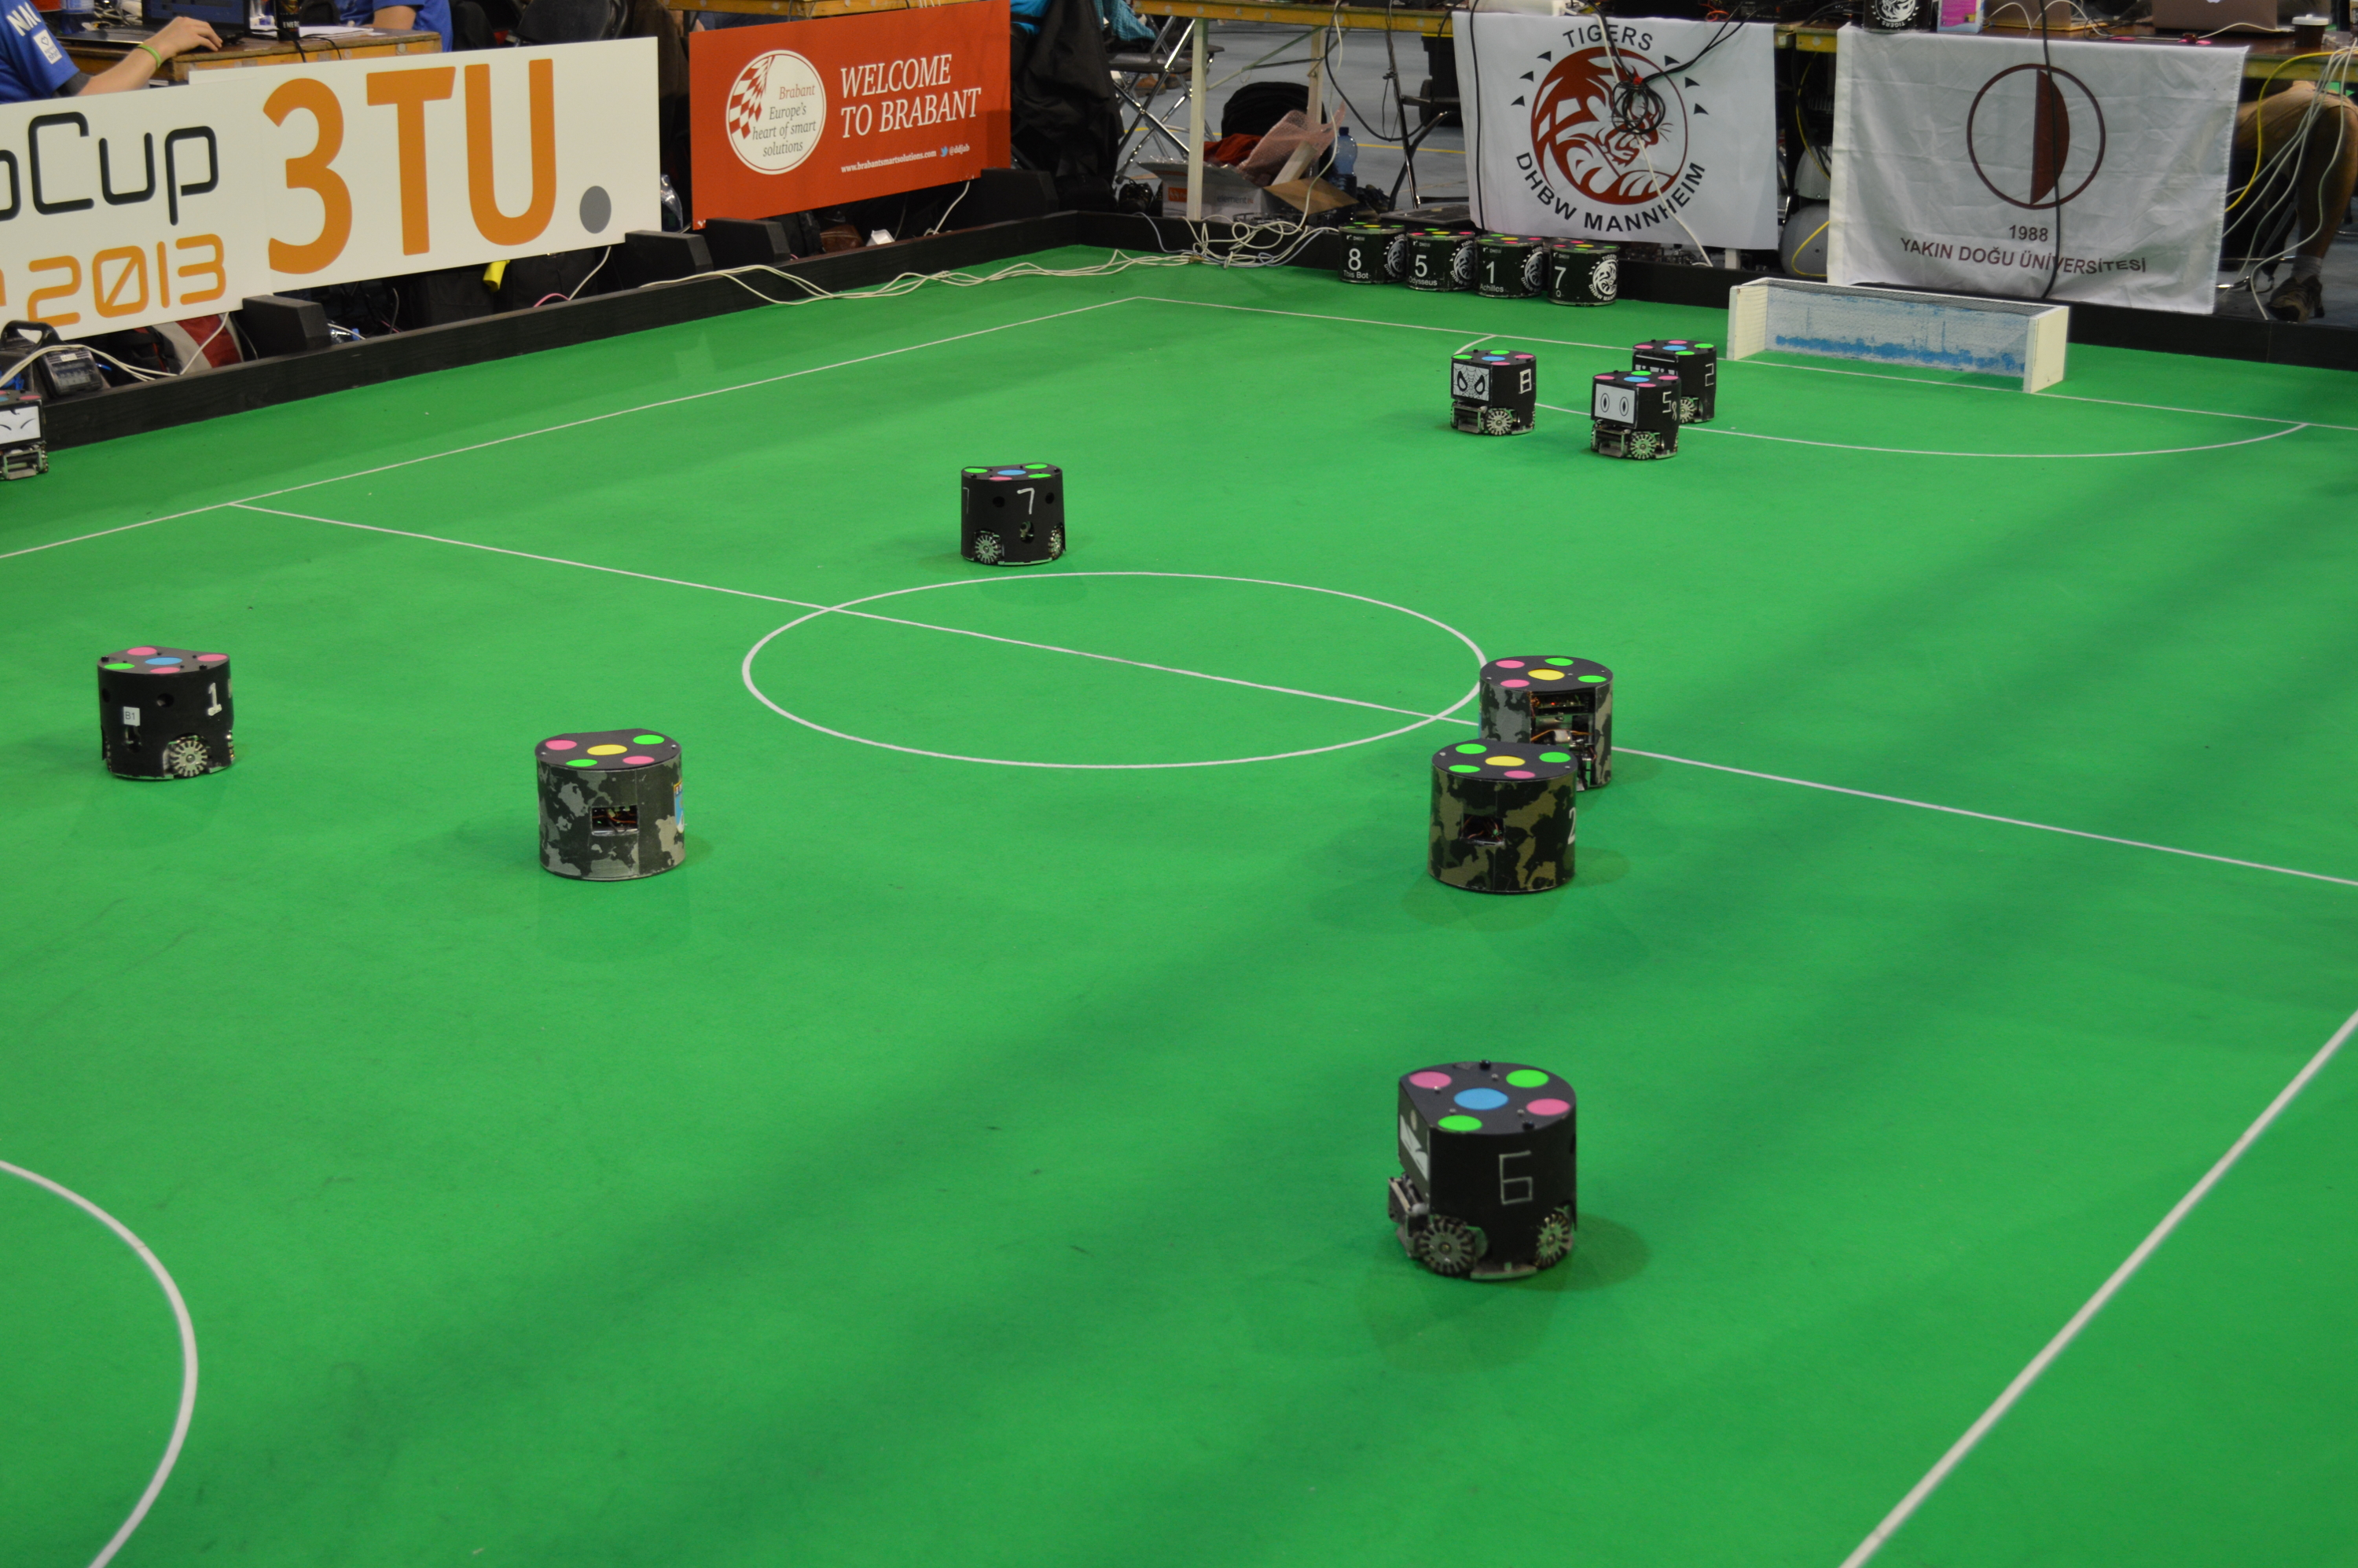
\includegraphics[width=0.8\linewidth]{robocup2013}
  \caption{Imagem da SSL \textit{RoboCup} 2013 em Eindhoven, na Holanda}\label{fig:robocup2013}
\end{figure}

Devido a alta complexidade desses ambientes, não é viável o planejamento
considerando diretamente as leis físicas. Como consequência, limita-se as ações
possíveis do robô no modelo utilizado no planejamento para que se possa simular
mais situações em tempo hábil, uma vez que o ambiente está continuamente sujeito
a modificações. Entretanto, para que as simulações sejam válidas, o robô real
deve estar em sintonia com seu modelo. Com efeito, o robô real deve executar os
comandos conforme o robô simulado, caso o mesmo ambiente simulado seja
encontrado na prática.

A ideia de robôs jogando futebol foi mencionada pela primeira vez pelo professor
Alan Mackworth (University of British Columbia, Canadá) em um artigo intitulado
"On Seeing Robots", apresentado no Vision Interface 92 e posteriormente
publicado em um livro chamado Computer Vision: System, Theory and Applications
\cite{basu1993computer}.  Independentemente, um grupo de pesquisadores japoneses
organizou um Workshop no Ground Challenge in Artificial Intelligence, em Outubro
de 1992, Tóquio, discutindo e propondo problemas que representavam grandes
desafios.
Esse Workshop os levou a sérias discussões sobre usar um jogo de futebol para
promover ciência e tecnologia. Estudos foram feitos para analisar a viabilidade
dessa ideia. Os resultados desses estudos mostram que a ideia era viável,
desejável e englobava diversas aplicações práticas. Em 1993, um grupo de
pesquisadores, incluindo Minoru Asada, Yasuo Kuniyoshi e Hiroaki Kitano,
lançaram uma competição de robótica chamada de Robot J-League (fazendo uma
analogia à J-League, nome da Liga Japonesa de Futebol Profissional). Em um mês,
vários pesquisadores já se pronunciavam dizendo que a iniciativa deveria ser
estendida ao âmbito internacional. Surgia então, a Robot World Cup Initiative
(RoboCup).

RoboCup é uma competição destinada a desenvolver os estudos na área de robótica
e Inteligência Artificial (IA) por meio de uma competição amigável. Além disso,
ela tem como objetivo, até 2050, desenvolver uma equipe de robôs humanóides
totalmente autônomos capazes de derrotar a equipe campeã mundial de futebol
humano. A competição possui várias modalidades. Neste trabalho, será analisada a
Small Size Robot League (SSL), também conhecida como F180. De acordo com as
regras da SSL de 2015, as equipes devem ser compostas por 6 robôs, sendo um deles o
goleiro, que deve ser designado antes do início do jogo. Durante o jogo, nenhuma
interferência humana é permitida com o sistema de controle dos robôs. É
fornecido aos times um sistema de visão global e esses controlam seus robôs através de
máquinas próprias. O sistema de controle dos robôs geralmente é externo e recebe
os dados de um conjunto de duas câmeras localizadas acima do campo. Esse sistema
de controle processa os dados, determina qual comando deve ser executado por
cada robô e envia este comando através de ondas de rádio aos robôs.
% Embora seja permitido que as equipes utilizem sistemas próprios de visão, a
% maioria das equipes utiliza a visão centralizada.

\section{Motivação}

% TODO: ABRIR AQUI UMA SUBSEÇÃO DENOMINADA CONTEXTUALIZAÇÃO INICIAL E COLOCAR AS
%       SEÇÕES 2.1 E 2.2 CO IP COMO SUBITENS. ?????

O futebol de robôs, problema padrão de investigação internacional, reúne grande
parte dos desafios presentes em problemas do mundo real a serem resolvidos em
tempo real. As soluções encontradas para o futebol de robôs podem ser
estendidas, possibilitando o uso da robótica em locais de difícil acesso para
humanos, ambientes insalubres e situações de risco de vida iminente.  Há
diversas novas áreas de aplicação da robótica, tais como exploração espacial e
submarina, navegação em ambientes inóspitos e perigosos, serviço de assistência
médica e cirúrgica, além do setor de entretenimento. Essas áreas podem ser
beneficiadas com o desenvolvimento de sistemas multi robôs. Nestes domínios de
aplicação, sistemas de multi robôs deparam-se sempre com tarefas muito difíceis
de serem efetuadas por um único robô.  Um time de robôs pode prover redundância
e contribuir cooperativamente para resolver o problema em questão. Com efeito,
eles podem resolver o problema de maneira mais confiável, mais rápida e mais
econômica, quando comparado com o desempenho que único robô teria.

Devido a alta complexidade de sistemas multiagentes dinâmicos, torna-se
necessário um modelo simplificado para que sejam executadas o maior número de
simulações possível.  Caso seja possível uma discretização, ter-se-á um número
finito de casos para serem avaliados. Com isso, pode-se desenvolver um sistema
multi-agente baseado em utilidade. Assim, o computador passa a escolher parte
da estratégia com base na função utilidade escolhida.
%como o Minimax (discutido no Capítulo~\ref{cap:minimax}) para encontrar
%soluções ao problema.

Isso é mais desejável que um modelo heurístico de IA, onde as soluções são
criadas com base nos ambientes identificados pelos modeladores. Isso, pois a
modelagem puramente heurística limita o número de jogadas que se pode executar e
limita a capacidade que o computador tem de testar um grande número de possibilidades.
O resultado é que a qualidade das jogadas se limita a capacidade de quem cria as
heurísticas.

\section{Objetivo}

O objetivo deste trabalho é desenvolver uma ferramenta de representação
comportamental baseado em otimização para futebol de robôs.
%O objetivo deste trabalho é desenvolver um algoritmo de controle para o futebol
%de robôs que obtenha um desempenho melhor que o utilizado atualmente, de acordo
%com a performance em um conjunto de partidas.
A meta intermediária é criar um modelo discreto sequencial
para o problema do futebol de robôs. A partir desta
discretização, foi desenvolvida uma arquitetura de controle
que seleciona jogadas o mais próximas da jogada ótima possível,
de acordo com uma função de avaliação e dentro do tempo disponível
para o planejamento.

\section{Justificativa}
% TODO: incluir referências

Uma arquitetura de controle que simule os diversos ambientes dinamicamente de
maneira sequencial de um ambiente multiagente permite que várias jogadas sejam
criadas dinamicamente, diferentemente de uma arquitetura estática baseada somente
em heurística. Essa abordagem heurística é legada da maneira como estratégias
são planejadas nos times de futebol humano.

Com tal mecanismo é possível melhorar a IA em uso pela RoboIME para tomar
decisões que levem a resultados melhores e, como consequência, ganhar mais
partidas. Nenhuma equipe atualmente esta seguindo esta abordagem, mas os autores
acreditam que essa é uma linha de pesquisa promissora, já que se utiliza da
capacidade que o computador tem de simular várias possibilidades em um curto
intervalo de tempo.

\section{Metodologia}

Para atingir os objetivos propostos será seguida a seguinte metodologia.
Inicialmente é criado um modelo sequencial do problema do futebol de robôs.
Para isso, a arquitetura do futebol de robôs considerada neste trabalho é
detalhada, juntamente com definições de termos relevantes para este trabalho.
% TODO: Mostrar os passos do trabalho, e não do relatório
%
%Um modelo abstrato do futebol de robôs é proposto para simplificar o problema
%e permitir que sejam feitas várias simulações durante o planejamento das
%jogadas. A função de avaliação, essecial para a seleção das jogas, é detalhada.
%
%Posteriormente a arquitetura da ferramenta a ser construida é apresentada.
%Os diversos componentes do sistema são detalhados.
%
%Em seguida, os resultados experimentais obtidos com a ferramenta detalhada
%anteriormente são apresentados.
%
%São apresentadas sugestões para trabalhos futuros e as principais dificuldades
%enfrentadas pelos autores são destacadas.
%
%Finalmente são apresentadas as conclusões do projeto.

\section{Estrutura}

% modelagem
No Capítulo~\ref{cap:modelagem}, um modelo do futebol de robôs é proposto.
Também é apresentada a função de avaliação.

% arquitetura
No Capítulo~\ref{cap:arquitetura}, a ferramenta proposta é desenvolvida com
base no modelo proposto anteriormente.

% resultados
No Capítulo~\ref{cap:resultados}, são apresentados os resultados obtidos
neste trabalho.

% considerações finais
No Capítulo~\ref{cap:cons_finais}, são apresentadas sugestões para trabalhos
futuros e as principais dificuldades enfrentadas pelos autores são destacadas.

% conclusao
Finalmente, são apresentados os principais resultados atingidos neste trabalho.

% vim: tw=80 et ts=2 sw=2 sts=2 ft=tex


% Desenvolvimento
% ---------------

\chapter{Minimax}\label{cap:minimax}

Minimax é um algoritmo que visa minimizar a perda máxima, isto é, dentre
o pior caso de cada possível decisão aquele que levar ao menor prejuízo.
Originalmente formulado para um jogo de soma zero de dois jogadores, o Minimax
já foi estendido para jogos mais complexos e decisões gerais em situações de
incerteza.

O princípio do minimax se aplica a um jogo $\Gamma=\langle A,B,H\rangle$ se a
equação~\ref{eq:req} for satisfeita, isto é, se existe uma valoração $v$ para o
jogo e uma estratégia ótima para ambos jogadores.
\cite{hazewinkel2002encyclopaedia}

\begin{gather}
  v=\max_{a\in A}\min_{b\in B}H(a,b)=\min_{b\in B}\max_{a\in A}H(a,b)\label{eq:req}
\end{gather}

Em que $A$ e $B$ são as estratégias dos jogadores 1 e 2 respectivamente e $H$ é a
função de utilidade que é positiva quando o jogador 1 está ganhando.

% TODO: explicar funcionamento
% TODO: Mostrar pseudo código

O algoritmo~\ref{lst:minimax} é um exemplo de pseudocódigo para o Minimax.

\begin{algorithm}
  \SetKwBlock{Procedimento}{Procedimento}{fim}
  \SetKwFunction{Utilidade}{Utilidade}
  \SetKwFunction{Proximos}{Próximos}
  \SetKwFunction{Valor}{Valor}

  \Entrada{$estado$, $jogador \in \{MIN, MAX\}$}
  \Saida{$decisão \in$ possíveis próximos estados}

  \Valor{$estado, jogador$} := \Inicio{%
    \Se{$estado$ é final}{%
      \Retorna{\Utilidade{$estado$}}\;
    }

    \eSe{$jogador$ = MAX}{%
      $valor \leftarrow$ máximo de $\Valor{proxEstado, MIN}: proxEstado \in \Proximos(estado)$\;
    }{% senão
      $valor \leftarrow$ mínimo de $\Valor{proxEstado, MAX}: proxEstado \in \Proximos(estado)$\;
    }
    \Retorna{$valor$}\;
  }

  \eSe{$jogador$ = MAX}{%
    $decisão \leftarrow proxEstado$ com máximo \Valor{$proxEstado, MIN$}\;
  }{% senão
    $decisão \leftarrow proxEstado$ com mínimo \Valor{$proxEstado, MAX$}\;
  }
  \Retorna{$decisão$}\;

  \caption{Pseudocódigo para tomada de decisão com o Minimax.}\label{lst:minimax}
\end{algorithm}

\section{Exemplo}

%A figura~\ref{fig:minimax-tree} exemplifica uma árvore de decisão usando esse
%método.
%
%\begin{figure}[ht]
%  \centering
%  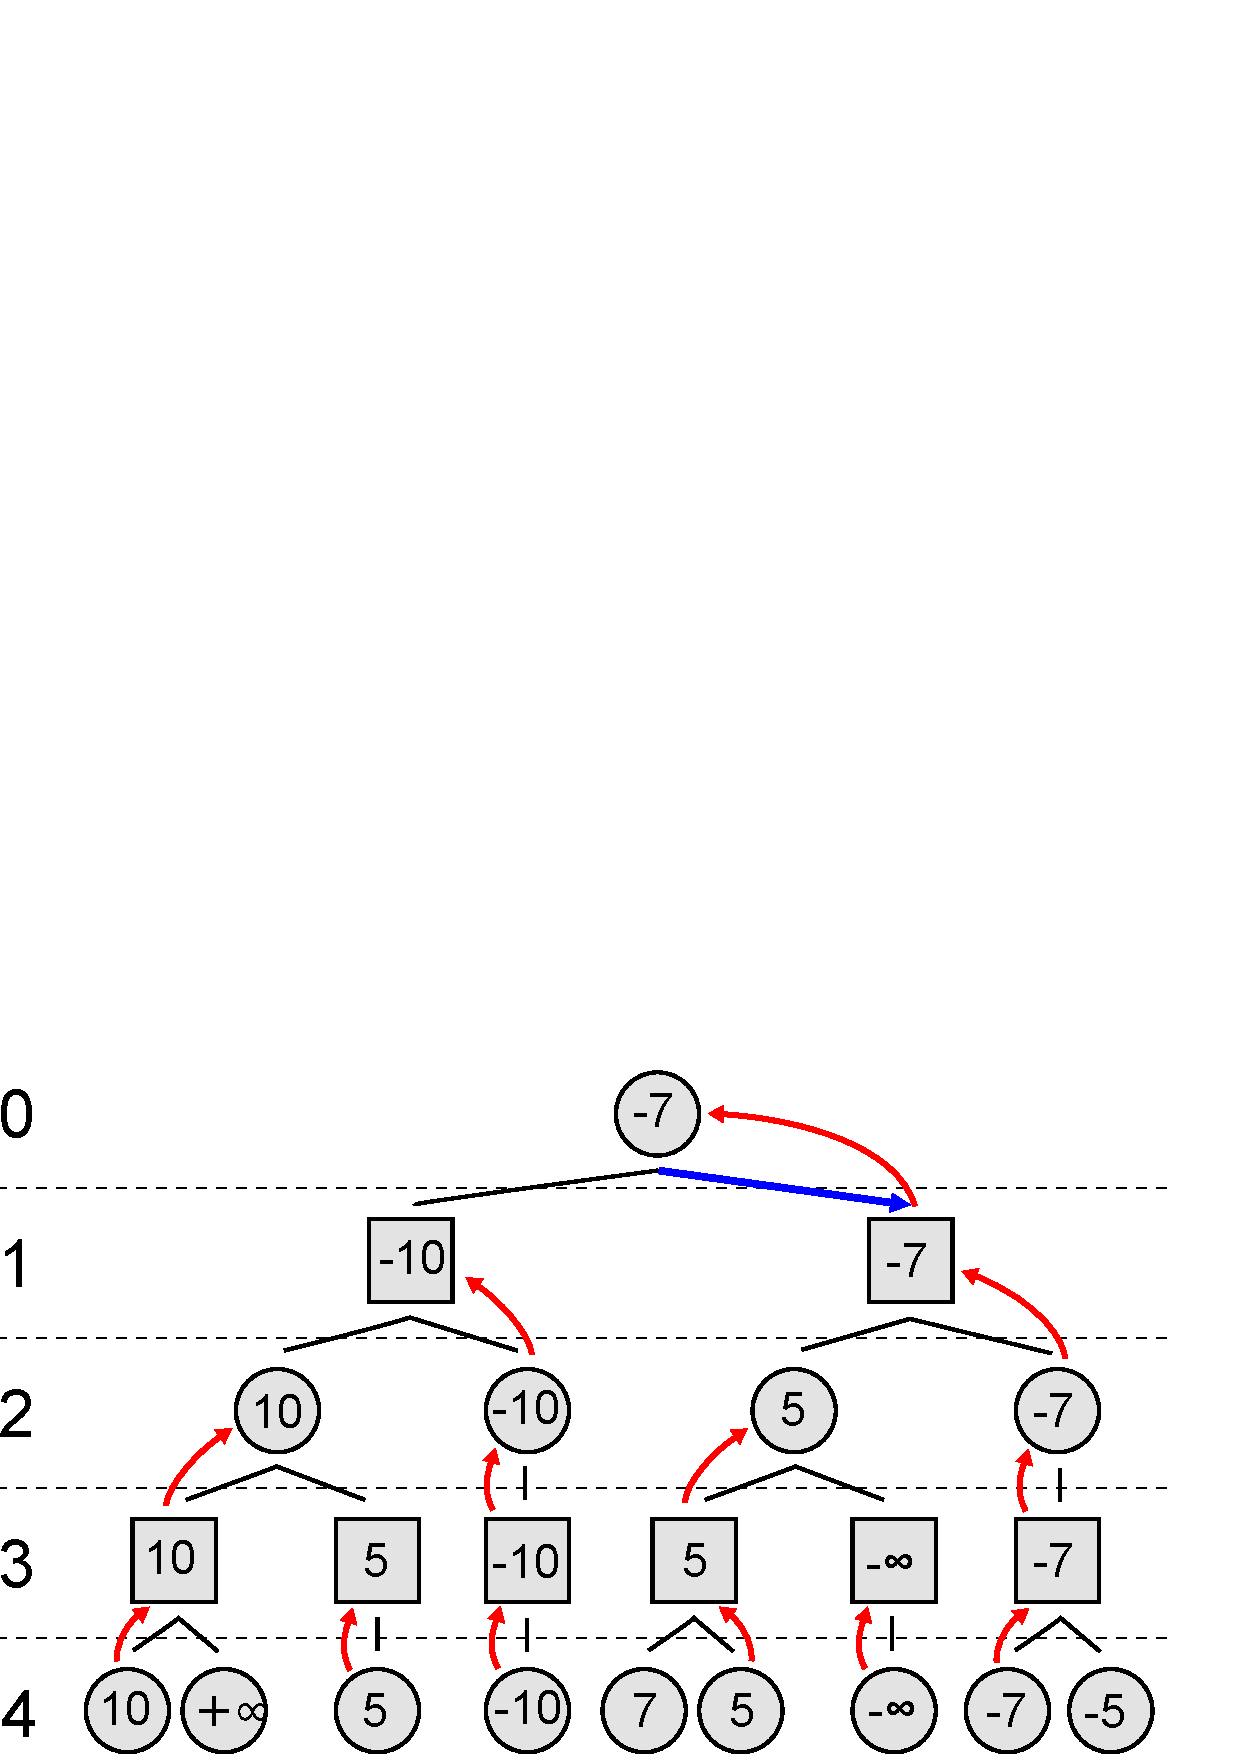
\includegraphics[width=0.7\linewidth]{minimax-tree}
%  \caption{Exemplo de árvore de decisão com Minimax.}\label{fig:minimax-tree}
%\end{figure}

O conhecido jogo da velha, que pode ser usado para exemplificar o algoritmo,
está representado na figura~\ref{fig:minimax-tictactoe}. Em que um valor $+1$
sinaliza uma vitória para o jogador $X$, $-1$ para o jogador $O$ e $0$, um
empate (ou velha).  Isto é o jogador $X$ é o $MAX$ e portanto $O$ o $MIN$.

Após aberta a árvore de jogadas e cada folha avaliada, nesse caso a avaliação
não é heurística pois o jogo é simples o suficiente para que isso não seja
necessário. A partir das folhas cada nó têm seu valor como o máximo dos valores
dos filhos quando é um nó $MAX$, e o mínimo quando $MIN$.

Assim a jogada imediata decidida pelo Minimax é a que tem valor $0$. Em termos
simplificados significa a jogada que na pior das hipóteses irá terminar em
velha.

\begin{figure}
  \centering
  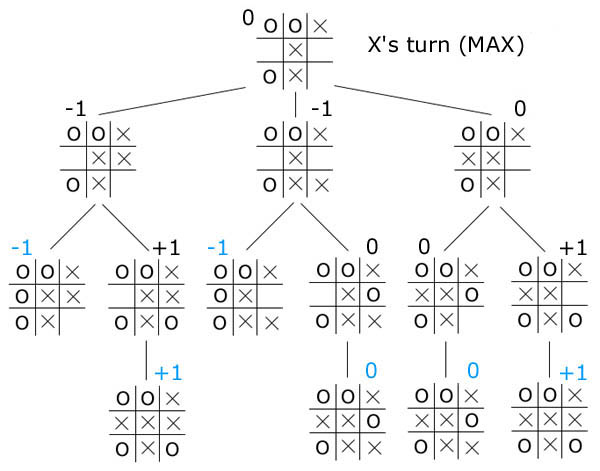
\includegraphics[width=0.7\linewidth]{minimax-tictactoe}
  \caption{Árvore do Minimax para o jogo da velha.}\label{fig:minimax-tictactoe}
\end{figure}

% vim: tw=80 et ts=2 sw=2 sts=2

\chapter{Mapeamento de jogo contínuo para um jogo discreto}\label{cap:mapeamento}

\section{Introdução}
% TODO[improvement]: add pictures for better understanding
Uma das dificuldades de se discretizar um sistema é a necessidade de criar uma abstração válida para
o jogo, de modo que o que ocorra na simulação acontessa na prática caso a mesma situação simulada
seja observada no mundo físico.

Essa modelagem pode ser separada em duas etapas:

\begin{itemize}
  \item Representação do jogo
  \item Execução do planejamento
\end{itemize}

\section{Representação do jogo}

Cada um dos robôs em campo será modelado com as seguintes ações possíveis:
\begin{itemize}
  \item Time com a bola
  \begin{itemize}
    \item robô sem a bola
    \begin{itemize}
       \item Move
    \end{itemize}
    \item robô com a bola
    \begin{itemize}
       \item Move
       \item Chute
       \item Passe
    \end{itemize}
  \end{itemize}
  \item Time sem a bola:
  \begin{itemize}
    \item Move
    \item GetBall
  \end{itemize}
\end{itemize}

O nível de complexidade das ações possíveis influi diretamente no número de ações que poderão
ser consideradas a tempo de serem úteis para o jogo real. Por exemplo, caso não fosse considerada
a ação de passe, esta ação ainda sim poderia acontecer na prática. Entretanto, seriam necessários
mais níveis de planejamento, uma vez que ela seria a composição de chutes e passes. Isso tem a
contrapartida de reduzir o número de estados que podem ser simulados, uma vez que o tabuleiro
é dinâmico e de o jogo real ser simultâneo, e não sequencial. Isso fica mais evidente se fossem
utilizadas somente as \textit{skills} para o planejamento. A principal desvantagem disso é que
o planejador teria que considerar aspectos como colisões e a orientação dos robôs no planejamento
final. Além de ser ineficiente, coisas como posicionamento global dos robôs no campo não teriam
estados suficientes na árvore do jogo para serem úteis.

Outra questão que se deve ter em mente ao se modelar as ações básicas dos robôs é definir ações
muito complexas. Passando para a linguagem da arquitetura STP(\textit{Skill, Tactic Play}),
as \textit{plays}, e não \textit{tactics}, o espaço de jogadas seria muito limitado se
fossem utilizadas táticas muito complexa.

Como a complexidade é cuja base é o número de jogadas, isso não é um problema que pode ser
tratado simplesmente com o aumento da velocidade de processamento. Deve-se ajustar o nível
de abstração de acordo com os resultados obtidos nos teste práticos.

\section{Execução do planejamento}
% TODO[improvement]: specify add images

Esta etapa do modelo é responsável por converter o resultado do planejamento em comandos mais
concretos. Conforme evidenciado na seção anterior, é nesta parte que o planejamento de trajetória
deve ser levado em consideração. Esta parte que leva em consideração o modelo dinâmico do robô.
Como isso é um problema complexo, com o objetivo de focar o escopo da pesquisa no planejamento
de alto nível, será utilizada a arquitetura de controle do pyroboime.


%\chapter{Lições Aprendidas com Implementações Anteriores}
\chapter{Experiencia com Implementações Prévias}

\section{Abordagens}

As abordagens consideradas para criação de uma IA para a SSL são:
\begin{itemize}
 \item Heurística pura
 \item Otimização
 \item Baseada em Jogos
 \item Otimização com modelagem do oponente
\end{itemize}

\section{Objetivos de longo prazo}
Desenvolver uma inteligência que comece com uma solução baseada em jogos, que
gradativamente vai aprendendo o comportamento de seu oponente e vai se
transformando em uma inteligência baseada em otimização, na medida do possível, e
enquanto for necessário.

\section{Problemas aprendidos}
A implementação de uma abordagem baseada em jogos com uma simulação física complicada
tornava a resposta lenta, logo a qualidade da solução obtida em tempo real era inferior
àquela obtida por uma heurística pura.
Foi tentado um minimax com simulador físico, mas o custo computacional das simulações
associado ao cresciemento exponencial da árvore minimax não permite um controle eficiente
dos robôs em um ambiente dinâmico com agentes que não são controláveis.
Foi tentado um minimax com chaveamento de heurística, mas fracasou devido ao
custo computacional. Logo também optou-se por heurísticas puras nos
times com robôs omnidirecionais.

\section{Proposta de solução}
Explorar o fato de que no jogo com robôs omnidirecionais não são necessárias as
trajetórias elaboradas que o primeiro time usava.
Aproximar a simulação física por um jogo de tabuleiro. Ou seja, levar a simulação para um
nível mais conceitual.

\section{Minimax para robôs omnidirecionais}
Modelagem das jogadas possíveis de cada robô:
\begin{itemize}
 \item Pegar a bola parada, se o oponente não estiver mais próximo da bola que o
 nosso robô.
 \item Pegar a bola em movimento, se for possível, escolhendo um ponto aleatório
 da trajetória da bola.
 \item Passar a bola, se não tiver ninguém que possa interceptar a bola.
 \item Chutar a gol, se não tiver ninguém no caminho da bola.
 \item Deslocar-se para outro ponto escolhido aleatoriamente, se não tiver ninguém
 em seu caminho, ou utilizar a célula de Voronoi.
 \item Deslocar-se para o ponto escolhido na última jogada. ( Aprendizagem local )
\end{itemize}

\section{Problemas}
Não foi realizado um mapeamento do modelo conceitual para os
controles dos robôs. Não foi descoberto o problema.

Considere que o time que esteja se defendendo esteja na raiz da árvore MiniMax.
Neste caso, o goleiro deste time sempre conseguirá ficar entre a bola e o gol.

\section{Ideias}
Provavelmente é necessário fazer algum tipo de desacoplamento do comportamento dos
jogadores para melhorar o aproveitamento da CPU\@.
Talvez seja melhor definir algumas jogadas de movimento com finalidade especifica,
por exemplo, bloquear a bola defensivamente. O problema é o aumento do tempo de
processamento.

\section{Considerações}
O benefício da substituição das jogadas do oponente por jogadas aprendidas é duplo,
aumenta-se a efetividade das jogadas, e simultaneamente possibilita que o
número de jogadas consideradas possa aumentar. O problema de encontrar um
modelo para o comportamento do oponente é a parte mais desafiadora do projeto.

% vim: tw=80 et ts=2 sw=2 sts=2

\chapter{Cronograma}\label{cap:cronograma}

Para facilitar a compreensão do projeto, optou-se por dividir o projeto em módulos
que seguirão o cronograma apresentado na tablela~\ref{tab:crono}.

\begin{table}[ht]
\resizebox{\textwidth}{!}{
\begin{tabular}{|c|c|c|c|c|c|c|c|c|c|c|c|c|c|c|c|}
\hline
 Ano   & \multicolumn{5}{|c|}{2014} & \multicolumn{5}{|c|}{2015}\\
\hline
\rowcolor[gray]{.8} Tarefas & Ago & Set & Out & Nov & Dez & Jan & Fev & Mar & Abr & Mai \\
\hline
\hline
% ----  & Ago   & Set   & Out    & Nov    & Dez   & Jan   & Fev  & Mar  & Abr  & Mai  \\
 MMP    & \azck & \azck & \azck  & \azl   & \azl  & \azl  & \azl & \azl & \azl &  ·   \\
\hline 
 PVC    &  ·    & ·     & \vdck  & \vdck  & \vrd  & \vrd  & \vrd & \vrd & \vrd &  ·   \\
\hline 
 IMPARQ & ·     & ·     & \vduck & \vduck & \vdu  & \vdu  & \vdu & \vdu & \vdu &  ·   \\
\hline
 IMPALG & ·     & ·     & ·      & ·      & \vdd  & \vdd  & \vdd & \vdd & \vdd &  ·   \\
\hline 
 TST    &  ·    & ·     & ·      & ·      & ·     & ·     & \mr  & \mr  & \mr  &  ·   \\
\hline 
 RED    & \vmck & \vrm  & \vmck  & \vmck  & \vrm  & \vrm  & \vrm & \vrm & \vrm &  ·   \\
\hline 
 DEF    &  ·    & ·     & ·      & ·      & ·     & ·     & ·    & ·    & ·    & \ovd \\
\hline
\end{tabular}
}
\caption{Cronograma --- {\footnotesize MMP: Modelagem do mapeamento; PVC: Prova de conceito;
IMPARQ: Implementação da arquitetura; IMPALG: Implementação do Algoritmo; RED: Redação do
texto; TST: Testes; DEF: Defesa}\label{tab:crono}}
\end{table}

\begin{itemize}
  \item Estado atual: implementação do algoritmo em progresso.
  \item Legenda:
    \begin{itemize}
      \item Modelagem do mapeamento: discutido no capítulo~\ref{cap:mapeamento};
      \item Prova de conceito: implementar execução, pelo menos no simulador, do planejamento
            no formato que o algoritmo deve retornar.
      \item Implementação da arquitetura: implementar todo o programa incluindo um stub do
            algoritimo do minimax, isto é, o programa final a menos da corretude do algoritmo.
      \item Implementação do algoritimo: avançar o algoritmo ao ponto que a solução retornada
            esteja correta e prática, isto é, pode ser utilizada para uma partida real ou
            simulada.
      \item Testes: realização de testes em partidas e coleta de dados obtidos através das
            métricas estabelecidas na seção~\ref{sec:metricas}.
      \item Redação: Desenvolvimento da monografia.
      \item Defesa: Apresentação final do projeto em razão da VF de PFC.
  \end{itemize}
\end{itemize}
% vim: ts=2 sw=2 sts=2


% ---
% Finaliza a parte no bookmark do PDF, para que se inicie o bookmark na raiz
% ---
\bookmarksetup{startatroot}%
% ---

%\addcontentsline{toc}{chapter}{Conclusão}
%%\addcontentsline{toc}{chapter}{Conclusão}
\chapter{Conclusão}\label{cap:conclusao}

% TODO:
% OBS: - Recontextualizar trabalho
%      - Retificação do cumprimento dos objetivos
%      - Listagem das contribuições
%      - Trabalhos futuros

Este trabalho objetiva desenvolver uma ferramenta de representação
comportamental baseada em otimização para futebol de robôs.  A meta
intermediária é criar um modelo discreto sequencial para o problema do futebol
de robôs. A partir desta discretização, foi desenvolvida uma arquitetura de
controle que seleciona jogadas o mais próximo da jogada ótima possível, de
acordo com uma função de avaliação e dentro do tempo disponível para o
planejamento.

Foi desenvolvido um modelo abstrato do futebol de robôs no
Capítulo~\ref{cap:modelagem}. Este modelo foi base para o programa apresentado
no Capítulo~\ref{cap:arquitetura}.

A ferramenta criada atingiu os objetivos desejados, modificando o comportamento
do time através da modificação dos parâmetros da função objetivo, conforme
mostrado no Capítulo~\ref{cap:resultados}. Também foi desenvolvida com sucesso
uma interface gráfica que permite modificar esses parâmetros em tempo de
execução.

O trabalho atual pode permitir que um time melhor seja criado modificando-se os
parâmetros da função objetivo ou adicionando novos custos à função objetivo.
Através do fornecimento dos parâmetros vencedores da competição anterior, tem-se
um avanço no desempenho do time.

Pode-se melhorar o time utilizando uma maneria automática para realizar as
partidas e avaliar o desempenho do time nessa partida. Isso permitiria que
algorítimos de otimização também fossem utilizados para melhorar os parâmetros.
Para isso, é a necessário um juíz automático para permitir jogos não
supervisionados por humanos.
% TODO: Escolher outra palavra, 'humanos' parece estranho.

% vim: tw=80 et ts=2 sw=2 sts=2 ft=tex


% ----------------------------------------------------------
% ELEMENTOS PÓS-TEXTUAIS
% ----------------------------------------------------------
\postextual


% ----------------------------------------------------------
% Referências bibliográficas
% ----------------------------------------------------------
%\bibliographystyle{plainnat}%abbrvnat, unsrtnat, apsrev, rmpaps, IEEEtranN, achemso, rsc
\bibliography{referencias}

% ----------------------------------------------------------
% Glossário
% ----------------------------------------------------------
%
% Consulte o manual da classe abntex2 para orientações sobre o glossário.
%
%\glossary

% ----------------------------------------------------------
% Apêndices
% ----------------------------------------------------------

% ---
% Inicia os apêndices
% ---
%\begin{apendicesenv}

% Imprime uma página indicando o início dos apêndices
%\partapendices

% ----------------------------------------------------------
%\chapter{Quisque libero justo}
% ----------------------------------------------------------
%\end{apendicesenv}
% ---


% ----------------------------------------------------------
% Anexos
% ----------------------------------------------------------

% ---
% Inicia os anexos
% ---
%\begin{anexosenv}

% Imprime uma página indicando o início dos anexos
%\partanexos

% ---
%\chapter{Morbi ultrices rutrum lorem.}
% ---

%\end{anexosenv}

%---------------------------------------------------------------------
% INDICE REMISSIVO
%---------------------------------------------------------------------

\printindex

\end{document}
% vim: tw=80 et ts=2 sw=2 sts=2
